\documentclass{article}

\usepackage{a4wide,amsmath,amssymb,fancyhdr,graphicx,tabularx,xspace, algorithmic,amsmath,color,dsfont}

\pagestyle{fancy}
\chead{}
\lhead{TU Eindhoven}
\rhead{Algorithms (2IL15) --- Homework Exercises}
\cfoot{\thepage}
\lfoot{}
\rfoot{}

%to include IPE/pdf correctly
\expandafter\ifx\csname pdfoptionalwaysusepdfpagebox\endcsname\relax\else
\pdfoptionalwaysusepdfpagebox5
\fi

%comments command
\newcommand{\complain}[1]{\begin{quotation} {\sf *** #1 ***} \end{quotation}}


%
% Macros
%


\newcommand{\Reals}{{\Bbb R}}
\newcommand{\Nats}{{\Bbb N}}
\newcommand{\Ints}{{\Bbb Z}}


\newcommand{\C}{\ensuremath{\mathcal{C}}}
\newcommand{\E}{\ensuremath{\mathcal{E}}}
\newcommand{\F}{\ensuremath{\mathcal{F}}}
\newcommand{\G}{\ensuremath{\mathcal{G}}}
\newcommand{\U}{\ensuremath{\mathcal{U}}}

\newcommand{\tree}{\ensuremath{\mathcal{T}}}
\newcommand{\node}{\nu}
\newcommand{\lchild}{\mathrm{lc}}
\newcommand{\rchild}{\mathrm{rc}}
\newcommand{\size}{\mathit{size}}
\newcommand{\leaf}{\mu}
\newcommand{\mylist}{{\cal L}}
\newcommand{\myroot}{\mathit{root}}
\newcommand{\key}{\mathit{key}}
\newcommand{\bd}{\partial}





\newcommand{\eps}{\varepsilon}
\newcommand{\ol}{\overline}
\renewcommand{\leq}{\leqslant}
\renewcommand{\geq}{\geqslant}



\newcommand{\pr}[1]{\Pr[#1]}
\DeclareMathOperator{\expectation}{E}
\newcommand{\expt}[1]{\expectation[#1]}
\newcommand{\events}[1]{\mbox{Events}(#1)}
\newcommand{\rank}{\mathit{rank}}
\newcommand{\result}{\mathit{result}}
\newcommand{\piv}{\mathrm{piv}}
\newcommand{\myexp}{\mathrm{exp}}
\newcommand{\best}{\mathrm{best}}
\newcommand{\worst}{\mathrm{worst}}
\newcommand{\dest}{\mathit{dest}}
\newcommand{\dist}{\mathit{distance}}
\newcommand{\weight}{\mathit{weight}}
\newcommand{\alg}{{\sc Alg}\xspace}

\newcommand{\start}{\mathit{start}}
\newcommand{\myend}{\mathit{end}}
\newcommand{\free}{\mathit{free}}

\newcommand{\etal}{{\emph{et al.}\xspace}}
%%
% Theorem-Like Environments
%
\newtheorem{defin}{Definition}
  \newenvironment{mydefinition}{\begin{defin} \sl}{\end{defin}}
\newtheorem{theo}[defin]{Theorem}
  \newenvironment{mytheorem}{\begin{theo} \sl}{\end{theo}}
\newtheorem{lem}[defin]{Lemma}
  \newenvironment{mylemma}{\begin{lem} \sl}{\end{lem}}
\newtheorem{propo}[defin]{Proposition}
  \newenvironment{myproposition}{\begin{propo} \sl}{\end{propo}}
\newtheorem{coro}[defin]{Corollary}
  \newenvironment{corollary}{\begin{coro} \sl}{\end{coro}}
%\newtheorem{obse}[defin]{Observation}
%  \newenvironment{observation}{\begin{obse} \sl}{\end{obse}}
%\newtheorem{rem}[defin]{Remark}
%  \newenvironment{remark}{\begin{rem} \rm}{\end{rem}}


\newenvironment{myproof}{\emph{Proof.}}{\hfill $\Box$ \medskip\\}

\newcommand{\blb}{]}
\newcounter{rcounter}
\newenvironment{rlist}%
{\begin{list}{A.1-\arabic{rcounter}}{\usecounter{rcounter}}}{\end{list}}
\newcounter{rcountermem}

%%%%%%%%%%%%%%%%%%%%%%%%%%%%%%%%%%%%%%%%%%%%%%%%%%%%%%%%%%%%%%%%%%%%%

\title{}
\author{Mart Pluijmaekers}
\date{15-5-2012}





%%%%%%%%%%%%%%%%%%%%%%%%%%%%%%%%%%%%%%%%%%%%%%%%%%%%%%%%%%%%%%%%%%%%%%%%%%%

\begin{document}

\section*{Algorithms (2IL15): Homework Set A}

\subsection*{Backtracking}
\begin{itemize}
\item[1.]\begin{algorithmic}[1]
\STATE{Powerset($n,a,b$)}
\STATE{print $b$}\ \ \ \ \ \ \ \ \ \ \ \ \ \ \ \ \ \ \ \ \ \ \ \ \ \ \ \ \ \ \ \ \ \ \ \ \ \ \ \ \ \ (this statement prints the contents of set $b$)
\FOR{$i \gets a$ to $n$}
	\STATE{Powerset($n, i+1, b \cup \{i\}$)}
\ENDFOR
\end{algorithmic}
The initial call to this algorithm is Powerset($n, 1, \{\}$).

Parameters:
\begin{itemize}
\item{$n$} Since we have to compute the powerset of the set $\{1,...,n\}$ we need a parameter to give us this maximal element, this is $n$.
\item{$a$} Since we added elements to the current working set (see the next item) we need to have a parameter which holds this information. $a$ thus gives us knowledge of the where we are, it dictates the lower end of the set. So we actually compute the powerset of the set $\{a+1,...,n\}$
\item{$b$} This is the working set, we have to keep this in order to know which set we have computed before, this can be seen as a sort of prefix 
\end{itemize}

The problem we are trying to solve is the following, compute the powerset of the set $\{a,...n\}$ and take the union with set $b$. This means that we look at $b$ like a prefix. The combination of $b$ and $a$ prevents us from computing sets twice, since all elements in $b$ are less then $a$.

\item[2.] 
\begin{itemize}

\item[(i)]
\begin{algorithmic}[1]
\STATE{count($S,X$)}
\STATE{$s \gets [0,0,0,0]$}
\FOR{$i \gets 1$ to length $S$}
	\STATE{$s[S[i]] \gets s[S[i]]+X[i]$}
\ENDFOR
\RETURN{$s[1]=s[2]=s[3]=s[4]$}
\end{algorithmic} 

\bigskip

\begin{algorithmic}[1]
\STATE{4Partition($X,S,h$)}
\IF{$n=$ length $S$ and count($S,X$)}
	\STATE{Print('YES')}
	\RETURN{\TRUE}
\ELSE
	\RETURN{\FALSE}
\ENDIF
\FOR{$i \gets n$ to length $X$}
	\FOR{$j \gets 1$ to $4$}
		\STATE{$S[i]=j$}
		\IF{4Partition($X,S,h+1$)}
			\RETURN{\TRUE}
		\ENDIF
	\ENDFOR
\ENDFOR
\IF{$n=1$}
	\STATE{Print('NO')}
\ENDIF
\end{algorithmic}

The initial call is 4Partition($X,S,1$) where $X$ and $S$ are the sets given in the assignment. ($S[i]$ depicts in what subset $X[i]$ is)\\

We have 3 parameters: $X$ contains the set which holds the elements that need to be partitioned. $S$ (like already explained) contains the information for every element of $X$ in which subset it resides. $h$ contains the current position of were the algorithm is at processing $X$.

The meaning of the parameters: We have 5 parameters, the first (\emph{total}) is the set on which we have to calculate whether a 4 partition does exist. The other four arguments (\emph{$a1,a2,a3,a4$}) contain the 4 candidate partitions. We add an element to these sets and recurse, in order to find all possible subsets and we thus get to see all valid 4 partitions.

The subproblem we try to solve is as follows, compute all possible partitions of a (sub)set $S$. We compute it for $<S_h,...,S_n>$ where $n$ is the length of $S$. In other words, we compute the partitioning of the set $X$ for all elements of $X$ where it's position in $X$ is greater or equal to $h$.

\item[(ii)] The recurrance is as follows:
      \[
      T(n) = \left\{
                   \begin{array}{ll}
                     1   & \mbox{if $|n|=0$} \\
                     n * 4 * T(n-1) & \text{otherwise}
                   \end{array}
                \right.
      \]
We prove the recurrence holds by induction on $n$.

\textbf{Base:} If $|n|=0$ then this would mean that the input set is empty, we then know that there ofcourse is a valid partition, since no elements partitioned into 4 sets gives 4 empty sets, which ofcourse have the same sum. \\

\textbf{Step:} When drawing the call tree we deduced that the algorithm probably had a running time, somewhere in the order of $c * n * 4^n$ (IH).
\begin{align*}
T(n) &= n * 4 * T(n-1) \\
&\le n * 4 * (c*(n-1)*4^{n-1})\ (IH)\\
&\le c*n * (n-1) *4 *4^{n-1}\\
&\le c*n*4^n
\end{align*}

So, we know our assumption was correct. This gives us a (worst case) running time in the order of $O(c*n*4^n)$ since $c$ is a constant we know we can omit this from the running time so we get a running time in the order of $O(n*4^n)$


\end{itemize}
\end{itemize}

\subsection*{Greedy algorithms}
\begin{itemize}
\item[1.] 

\begin{itemize}	
\item[i] This does not hold, if we were to take a look at the following example. 

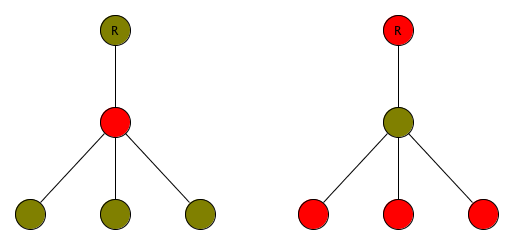
\includegraphics[scale=0.73]{greedy_graph.pdf}

In both graphs the roots have label \emph{R}. If we look at the left graph, it is coloured according to the scheme given in the exercise, the root is coloured green and all it's children are coloured red. Since the node on the second leven is red, all of it's children have to be green. But if we made the root red (like in the right graph), we have to make all (the node on the second level) of it's children green, but since we do not have any rules about green nodes, we can simply colour all the children of the node on the second level red. The left graph has 4 green nodes, while the right graph only has one. So the greedy choice made in the proposal is not valid.

\item[ii] This does hold. \\
Lemma: Let $v$ be a parent of a deepest node in $\mathcal{T}$. Then there is an optimal solution to the coloring problem for $\mathcal{T}$ for which $v$ is green.

Proof: Let $OPT$ be an optimal solution for $A$. If OPT has every parent of a deepest node green, then the lemma obviously holds, so assume OPT does have parents of deepest nodes which are not green. We show how to modify an optimal solution $OPT$ into solution $OPT^*$ such that
\begin{itemize}
\item[$(i)$] $OPT^*$ is a valid solution.
\item[$(ii)$] In $OPT^*$ $v$ is a green node. 
\item[$(iii)$] The number of green nodes in $OPT^*$ is $\le$ the number of green nodes in $OPT$.
\end{itemize}
\end{itemize}

Thus $OPT^*$ is an optimal solution having every parent of the deepest nodes green and so the lemma holds. To modify OPT we proceed as follows.

Let $v$ be a node in $\mathcal{T}$ which is the parent of a deepest node and let $OPT^*$ be equal to $OPT$ but $v_{OPT^*}$ is colored green. We now have 2 distinct possibilities, either $v_{OPT}$ is green, or it is red.

\begin{itemize}
\item[$v_{OPT}$ is green] If it was green then we are done, $(i)$ holds since we did not change $OPT$ in order to get $OPT^*$ so $OPT^*$ is a valid solution. $(ii)$ holds since the $v$ is a green node. and $(iii)$ holds since we did not change the number of green nodes in $OPT^*$ compared to $OPT$ so the number of green nodes remains the same.
\item[$v_{OPT}$ is red] Then this automatically means by definition that all of $v_{OPT}$ children are  green. Atleast, if it has children, if it does not have children it means that it is the root, which by definition does not have a parent, so it is colored red. If we then change $v_{OPT}$ to green by the greedy choice we can make all of it's children red. $(i)$ holds, since it is still a valid solution, the coloring of the parent of $v$ does not have to change (necciseraly) since we changed the color of $v$. $(ii)$ holds trivially, since this is what we changed. $(iii)$ also holds, let $n$ be the number of green nodes in $OPT$ and $m$ be the number of green nodes in $OPT^*$. Then $m$ is equal to $n+1$ since we turned $v$ from red to green, but since we now can color all of $v$'s children red we can also substract $\#children(v)$. This means that $m=n+1-\#children(v)$. $\#children(v)\ge 1$ since we know that $v$ is a parent and thus has atleast 1 child. Thus $m=n+1-\#children(v)\le n$. Note that this shows that when the parent of a deepest node is red and has more then 1 child. It cannot be optimal, since by changing this node to the colour green and all of its children to red, we lower the total number of green nodes. This means that the solution was not optimal to start with, which produces a contradiction so from this we have also proven that the greedy choice is valid.


\end{itemize}
We have shown that $(i),(ii)$ and $(iii)$ hold so we know that the choice of coloring the parent of a deepest node green is a valid greedy choice.

\newpage
\item[2.] 
\begin{itemize}
\item[i]
\begin{algorithmic}[1]
\STATE{CalcScheduling($A$)}
\STATE{$r1 \gets start(1)$}\ \ \ \ \ \ \ \ \ \ \ \ \ \ \ \ \ \ \ \ Initial starting time of room 1
\STATE{$r2 \gets start(2)$}\ \ \ \ \ \ \ \ \ \ \ \ \ \ \ \ \ \ \ \ Initial starting time of room 2
\STATE{$r3 \gets start(3)$}\ \ \ \ \ \ \ \ \ \ \ \ \ \ \ \ \ \ \ \ Initial starting time of room 3
\STATE{$A \gets sort(A)$}
\FOR{$i \gets 1$ to length($A$)}
	\STATE{$j \gets$\emph{room(number) with $r_j$ and $s(i)$ minimized, while $s(i)>r_j$ otherwise $nil$}}
	\STATE{$A[i]=j$}
	\IF{$j\ne NIL$}
		\STATE{$r_j=f(i)$}
	\ENDIF
\ENDFOR
\end{algorithmic}

For this algorithm we have provided pseudo code, here is a brief explenation about how it works. Firstly we initialize variables to contain the times the rooms become available, since we assumed that this was a variable which we had to update. Then we sort the input array according to the time the activities finish. The activity which finishes first is put on top, the second after that and so on (increasing). After that we look at each activity (in order) and schedule it in a room such that the waiting ``idle''-time of a room is minimized. Loop until all, activities have been assigned to a room (or to $nil$). Then we have completed our scheduling.

\item[ii] First we give the proof of the greedy choice, then we give a proof of the algorithm itself.\\
\textbf{Lemma:} Let $a_i$ be an activity in $A$ that ends first then there is an optimal solution to the Scheduling problem for $A$ that includes $a_i$ \\

\textbf{Proof:} Let $OPT$ be an optimal solution for $A$. If $OPT$ includes $a_i$ then the lemma obviously holds, so assume $OPT$ does not include $a_i$. We will show how to modify $OPT$ into a solution $OPT^*$ such that:
\begin{itemize}
\item[(i)] $OPT^*$ is a valid solution.
\item[(ii)] $OPT^*$ includes $a_i$.
\item[(iii)] $OPT^*$ is at least as good as $OPT$, which means size($OPT^*)\ge $size($OPT$)
\end{itemize}

Thus $OPT^*$ is an optimal solution including $a_i$ and so the lemma holds. To modify OPT we preseed as follows. Let $a_k$ be an activity in $OPT$ ending first and let $OPT^*=(OPT \setminus \{a_k\}) \cup \{a_i\}$. Then $OPT^*$ includes $a_i$ and size($OPT^*$)=size($OPT$). 
We then have 2 distinct possibilities, either $s(i) \ge s(k)$ or $s(i) < s(k)$. Note we have that end($a_i) \le $end($a_k$) by definition of $a_i$, so that $a_i$ cannot overlap any activities in $OPT \setminus \{a_k\}$.

\begin{itemize}
\item[$s(i)\ge s(k)$] If this is true, it means that the start time of activity $A[i]$ is at a later point in time. Since we have that end($a_i) \le $end($a_k$) we know we have a valid solution when there is no overlap, since $s(i) \ge s(k)$ the duration of this activity has the same or a later start time and an earlier ending time so cannot overlap with any other possible activity in the room $a_k$ was scheduled in, in $OP$.
\item[$s(i) < s(k)$] If this holds it means that the start time of $A[i]$ is earlier then the start time of $A[k]$. Because of this we again end up with 2 distinct possibilities. Let $h$ be the roomnumber $a_k$ was scheduled in. Then it is possible that start$(h)\le$start($A[i]$) or start$(h) > $start($A[i]$).

\begin{itemize}
\item[start($h) \le$ start($A[i\blb$)] Then we are finished immediately, since we know that end($a_i) \le $end($a_k$) and we know that start($h) \le$ start($A[i\blb$), we know that $a_i$ still fits inside the void left by $a_k$.
\item[start($h$) $\textgreater$ start($A[i\blb$)] If this is the case then it is obvious that $a_i$ cannot fit in the void left by removing $a_k$ from $OPT$. So we have to modify $OPT^*$ as follows $OPT^{**}=(((OPT^*\setminus a_i )\cup a_k) \setminus a_v) \cup a_i$. $a_v$ is an activity for which $s(A[v])<s(A[i]), it obviously holds that $f(A[v\blb$)>f(A[i])$. Since the start time of $a_v$ is earlier then that of $a_i$ we can place $a_i$ in this slot. Note that if there does not exist an $a_v$ it is not possible to place $a_i$, but no possible scheduling can achieve the scheduling of an activity before something has become available so this does not pose a problem for the greedy choice.
\end{itemize}


\end{itemize}
We have showed that when the greedy choice is made (and a scheduling of that activity is possible) that it can be scheduled and the solution still is optimal.


We will prove the correctness of the algorithm by induction on $n$, the number of elements to be scheduled. We define 2 base cases, 0 and 1 activitie(s) and then the step is more then 1 activity.

Let $n$ be the number of activities to be scheduled. ($n=\text{length}(A)$)

\textbf{$n=0$} Then there are no activities to be scheduled, which will always give a correct and optimal solution.
\textbf{$n=1$} If there is only one activity to be scheduled we have 2 possibilities, either a room is available for it to be scheduled in or it is not available. Either way we know that the algorithm provides a valid and correct solution. This is because in the \emph{for} loop of lines $6-10$ we select the room which minimizes the ``idle''-time. If there is atleast one room available, it is scheduled in the room which minimzes this ``idle''-time. When no room can be found it is obvious that it will not get scheduled ($j$ will contain $NIL$). Either way we know for sure that the algorithm will schedule the available activity in an available room whenever this is possible.

\textbf{$n>1$} When we need to schedule more then one activity we can see that we loop over the activities after they are sorted, this means that we handle each activity by ending time in ascending order. Because of this we know that if we have scheduled activity $i$ that activity $i+1$ has an ending time which is the same or later as that of activity $i$. So let activity $i$ be scheduled by our algorithm. If we want to schedule $i+1$ we have three distinct possibilities. Firstly it is possible that we cannot find a room for the activity because all rooms are taken at the starting point of the activity. Since we have the constraint that the startingpoint of an activity has to be stricly greater then the time a room becomes available we know that in this case the value for $j$ will become $NIL$ meaning that it will not be scheduled which is ofcourse the intended behaviour. The second case is when we do have a room available, in this case it means that there is at least one room available with an available time of less then the start time of activity $i+1$. When this happens the algorithm chooses the room from the available rooms which minimizes the idle time. Since we know we can place them, $j$ will not be equal to $NIL$ and thus the activity will be scheduled. Note that in all cases that an activity can be scheduled ($j\ne NIL$) the availability time of the room is changed to the ending time of the activity last added and since this now is the time this room becomes available it is trivially seen that this is correct.

We have now proved that in all cases we have a correct scheduling of activities and thus our algorithm is correct.

\item[iii] When looking at the algorithm we can see that lines $1-5$ and $8-11$ take constant time since they are simple assignments

 If we take a look at the algorithm we can clearly see that lines $1-4,8$ and $9$ take a constant time to compute, since they are just assignments. Line 7 is a special case, here a room is chosen where the activity is going to be scheduled in. If we were to program this we could program it as a sequence of 4 if/else statements which would compute the room with minimal ``idle''-time between the time the room becomes available and the starting time of a activity. But let's just parameterize this 4 for now. This means that we can write this statement as a for loop, which has to run from 1 to $r$ where $r$ is the number of rooms we have available for scheduling. Line 5 is even more special, since this line depicts the sorting of $A$. Since we know from datastructures that we can sort using many different algorithms, all with different properties (heapsort, radixsort, mergsort, ...) which all have different worst-case running times we will pick pick one since we do not have a special case here. We simply want to sort a set of integers. We like mergesort because of it's nice running time and it's nice way of sorting. But any other sorting algorithm can be used in order to sort $A$, we did not choose radixsort on purpose, since it is possible that the times are depicted as reals in which case the sorting with radixsort can become quite tricky, so even though radixsort can sort in linear time we decided not to pick it because of the possibilities of reals. The total running time will then become $O(n\log{n}+n*r)$, since $n\log{n}$ depicts a higher running time then $n*r$ (because $r$ will most of the time be much less then $n$) the running time of the algorithm will be $O(n\log{n}$. (please note that if radixsort would be used to sort the finishing times we would get a running time in the order of $O(n)$)


\end{itemize}
\end{itemize}

\subsection*{Dynamic Programming}
\begin{itemize}
\item[1.] 
\begin{itemize}

\item[(i)] We want to compute the minimal cost for traveling distance $D$ along a highway and we know we have to (potentially) stop at a number of petrol stations. If we also make the start and end position into petrol stations, we have to compute the minimal time to travel from the first to the last petrol station while stopping for gas before the fuel runs out. A natural way to devide this into subproblems is as follows: Given $j$, try to calculate the optimal solution's value and a feasable sequence of petrol stations $S=\{p_0,...,p_n\}$ where $p_0$ is the first petrolstation we stop and $p_n$ the last. 

\item[(ii)]
      \[
      m[j] = \left\{
                   \begin{array}{ll}
                     t(j)   & \mbox{if $d_{max}+d(j)\le D$} \\
                     min\{ m[k] + t(j) : d(j) < d(k) \le d_{max} + d(j), j<k\le n\}  & \text{otherwise}
                   \end{array}
                \right.
      \]

For this proof we have to split the recurrence in the basecase and in the other case. (case distinction).

In the case of $d_{max}+d(j)\le D$ we know that the distance is reachable after station $i$ (which can also be the starting point, since we made this a petrol station too). Then it is trivial to see that the minimal waiting time is the waiting time at petrol station $i$. Since we can then continue to drive to the endpoint. Only tanking in petrol station $i$ will obviously result in a waiting time of $t(i)$.

In the other case we consider the optimal solution $OPT$ for computing a feasable sequence of petrol stations $<p_j,...,p_{n+1}>$ and let $k^*$ be the index such that $OPT$ is of the form $<s_{k^*},...,s_{n+1}>$ . Then:
\begin{align*}
m[j] &= (\text{cost in }OPT\text{ for }<s_{k^*},...,s_{n+1}>) + t(k^*) \\
&\ge m[k^*] + t(k^*)\\
&\ge min\{ m[k] + t(j) : d(j) < d(k) \le d_{max} + d(j), j<k\le n\}
\end{align*}

On the other hand, for any $d(j) < d(k) \le d_{max} + d(j)$ and $j<k\le n$, there is a solution of cost $m[k]+t(k)$, so $m[k] = min\{ m[k] + t(j) : d(j) < d(k) \le d_{max} + d(j), j<k\le n\}$.

\item[(iii)]
\begin{algorithmic}[1]
\STATE{calcMinDist($D,d_{max},t,d$)}
\STATE{$n \gets $ length $t$}
\STATE{$t[0] \gets 0$}
\STATE{$t[n+1] \gets 0$}
\STATE{$d[0]\gets 0$}
\STATE{$d[n+1] \gets D$}
\FOR{$j \gets 0$ \textbf{to} $n+1$}
	\STATE{$m[j] \gets d(i)$}
\ENDFOR
\FOR{$j \gets n+1$ \textbf{downto} $0$}
	\STATE{$m[j] \gets min\{m[k] + t(j) : d(j) < d(k) \le d_{max} + d(j), j<k\le n\}$}
\ENDFOR
\RETURN{$m[0]$}

\end{algorithmic}


\item[(iv)] For the running time we can trivially see that lines $1-6$ and $13$ take constant time, since they are simple assignments or a return statement. Lines $7-9$ depict a for loop, for which the body (line 8) has a constant running time. The for loop itself runs over $n$ so this gets $\sum_{j=1}^n{O(1)}$. We again got another loop, lines $10-12$ but in this case the body does not have a constant time operations in it's body. What happens is that a minimum is chosen from possibly $n$ elements. This is not obvious when looking at it for the first time, since the set which is checked is limited, since it only checks for petrol stations which can be reached. But since it is possible that all petrol stations can be reached before the fuel runs out, it is possible that we have to iterate $n$ times. In this hidden inner loop only checks and assignments (see the algorithm in subquestion 5) are done. This gives the following running time for this part: $\sum_{j=o}^n{\sum_{j=o}^n{O(n)}}$. By solving the sums we get $\sum_{j=1}^n{O(1)}=O(n)$ and $\sum_{j=o}^n{\sum_{j=o}^n{O(n)}}=\sum_{j=o}^n{O(n)}=O(n^2)$. This means that the worst case running time is in the order of $O(n^2)$.

\item[(v)] 
In order to compute this we have to expand the loop of line 11 of \emph{calcMinDist}

The pseudocode for the algorithm is.
\begin{algorithmic}[1]
\STATE{calcMinDistAns($D,d_{max},t,d$)}
\STATE{$n \gets $ length $t$}
\STATE{$ans \gets$ array of sets, array of length $n+2$ }
\STATE{t$[0] \gets 0$}
\STATE{t$[n+1] \gets 0$}
\STATE{d$[0]\gets 0$}
\STATE{d$[n+1] \gets D$}
\FOR{$j \gets 0$ \textbf{to} $n+1$}
	\STATE{$m[j] \gets d(i)$}
\ENDFOR
\FOR{$j \gets n+1$ \textbf{downto} $0$}
	\STATE{$k \gets j+1$}
	\STATE{$min \gets k$}
	\WHILE{$d(k)-d(j) < D$}
		\IF{$t(k) < t(min)$}
			\STATE{$min \gets k$}
		\ENDIF
		\STATE{$k \gets k+1$}
	\ENDWHILE
	\STATE{$m[j] \gets t(min)+t(j)$}
	\STATE{$ans[j] \gets ans[min] \cup \{j\}$}
\ENDFOR
\RETURN{$ans[0]$}
\end{algorithmic}
It works the same way as \emph{calcMinDist} does, except it contains an extra array containing the following information: for petrol station $j$, $ans[j]$ is equal to all petrol stations which provide an optimal solution for traveling from petrol station $j$ to petrol station $n+1$. (the end point) Since it now is required to not return the optimal value, but the optimal solution itself $ans[0]$, depicting the set of petrol stations visited to get an optimal solution for traveling from petrol station $0$ to petrol station $n+1$. This also means that we get 2 extra petrol stations, the both newly defined ones. These can be trivially removed but for the sake of clarity we left these in the returned solution.

\end{itemize}

\item[2.]
\begin{itemize}

\item[(i)] Given $i,j$ give a partitoning for which $i$ is the rightmost point of partition $P_1$ and $j$ is the rightmost point of partition $P_2$. This means that all points $p_h, h\ge max\{i,j\}$ still have to be assigned to a partition. The subproblem is to assign each $p_h$ (in order) to a partition such that $Cost(P_1)+Cost(P_2)$ is minimal.

\item[(ii)] The recurrence is as follows:
      \[
      m[i,j] = \left\{
                   \begin{array}{ll}
                     0   & \mbox{if $i=n \vee j=n$} \\
                     min\{|p_{h+1}p_{j}| + m[h+1,j], |p_ip_{h+1}| + m[i,h+1]\}& \text{otherwise}
                   \end{array}
                \right.
      \]
In this recurrence we used the variable $h$, $h$ contains the maximum of $i$ and $j$. Since we think that it is almost impossible to write this in a readable fashion we decided to do it this way.

\textbf{Proof:}\\
\textbf{$i=n \vee j=n$} This case is trivial, since we try to make an optimal partitioning starting at point $i$ or $j$ we can see that we cannot add anymore points to a partition so the cost at that stage is $0$.

\textbf{Other cases:} We have that $i$ and $j$ represent the right most points of their respective partitions, for the next elements of $p$ we are going to select were we can place each element best. Furthermore we need to know the cost of joining this new element ($p_{h+1}, h=max\{i,j\}$) to a partition, this means that we have to compute the cost for $p_h$ to $p_i$ and $p_j$. Since the minimal cost of partitioning further then $p_h$ is contained in $m[i,h+1]$ for the partition where $i$ is the rightmost element and $m[h+1,j]$ for the partition where $j$ is the rightmost element we get that the minimal cost required to finish the partitioning is equal to the minimal values of these 2 values (for each partition). Which gives us our recurrence.
\item[(iii)] 
\begin{algorithmic}[1]
\STATE{OptimalPartitioning($p$)}
\FOR{$i \gets 1$ to $n$}
	\STATE{$m[i,n]=0$}
	\STATE{$m[n,i]=0$}
\ENDFOR
\FOR{$i \gets n - 1$ downto $0$}
	\FOR{$j \gets n - 1$ downto $0$}
		\STATE{$h \gets max\{i,j\}$}
		\STATE{$m[i,j] \gets min\{|p_{h+1}p_{j}| + m[h+1,j], |p_ip_{h+1}| + m[i,h+1]\}$}
	\ENDFOR
\ENDFOR
\RETURN{$m[0,0]$}
\end{algorithmic}

\item[(iv)] For the running time analysis, if we can clearly see that lines $3,4,8,9$ and $12$ take linear time since they are simple assignments. On first glance one would think that line $9$ is a loop, but since it only entails a few lookups and selects the smallest it can be regarded as an if statement, which ofcourse has linear running time. Furthermore we have 3 for loops of which 2 are nested in eachother. The for loop of lines $2-4$ has runs over $n$ so it is $\sum_{i=1}^n{O(1)}=O(n)$. The pair of nested for loops of lines $6-11$ also run over $n$, this means that the time neccesary to compute equal is to $\sum_{i=0}^n{\sum_{j=0}^n{O(1)}}=\sum_{i=0}^n{O(n)}=O(n^2)$. Since we know that $n^2$ is asymptotically steeper then $n$, we know that the algorithm will be in the order of $O(n^2)$

\end{itemize}
\end{itemize}


\end{document} 